% induction.tex
% Updated January 11, 2012

\chapter{Induction}\label{ch:induction}
The twin concepts of recursion and induction are fundamentally
important in combinatorial mathematics and computer science.  In this
chapter, we give a number of examples of how recursive formulas arise
naturally in combinatorial problems, and we explain how they can be
used to make computations.  We also introduce the Principle of
Mathematical Induction and give several examples of how it is applied
to prove combinatorial statements.  Our treatment will also include
some code snippets that illustrate how functions are defined
recursively in computer programs.


\section{Introduction}\label{s:induction:intro}
A professor decides to liven up the next combinatorics class by
giving a door prize.  As students enter class (on time, because to be
late is a bit insensitive to the rest of the class), they draw a
ticket from a box.  On each ticket, a positive integer has been
printed.  No information about the range of ticket numbers is given,
although they are guaranteed to be distinct. The box of tickets was
shaken robustly before the drawing, so the contents are thoroughly mixed, 
and the selection is done without looking inside the box.

After each student has selected a ticket, the professor announces that
a cash prize of one dollar (this is a university, you know) will be
awarded to the student holding the lowest numbered ticket---from among
those drawn.

Must the prize be awarded?  In other words, given a set of positive
integers, in this case the set of ticket numbers chosen by the
students, must there be a least one?  More generally, is it true that
in any set of positive integers, there is always a least one?  What
happens if there is an enrollment surge and there are infinitely many
students in the class and each has a ticket?

\section{The Positive Integers are Well Ordered}\label{s:induction:posintsord}

Most likely, you answered the questions posed above with an
enthusiastic ``yes'', in part because you wanted the shot at the
money, but more concretely because it seems so natural.  But you may
be surprised to learn that this is really a much more complex subject
than you might think at first.  In \autoref{app:background}, we discuss
the development of the number systems starting from the Peano
Postulates.  Although we will not devote much space in this chapter to
this topic, it is important to know that the positive integers come
with ``some assembly required.''  In particular, the basic operations
of addition and multiplication don't come for free; instead they have
to be defined.

As a by-product of this development, we get the following
fundamentally important property of the set $\posints$ of positive
integers:

\medskip
\noindent\textbf{Well Ordered Property of the Positive Integers:}\quad 
Every non-empty set of positive integers has a least element.

\medskip 

An immediate consequence of the well ordered property is that the
professor will indeed have to pay someone a dollar---even if there are
infinitely many students in the class.

\section{The Meaning of Statements}\label{s:induction:statements}

Have you ever taken standardized tests where they give you the first
few terms of a sequence and then ask you for the next one? Here are
some sample questions.  In each case, see if you can determine a
reasonable answer for the next term.

\begin{enumerate}
\item $2,5,8,11,14,17,20,23,26,\dots$
\item $1,1,2,3,5,8,13,21,34,55,89,144,233,377,\dots$
\item $1,2,5,14,42,132,429,1430,4862,\dots$
\item $2,6,12,20,30,42,56,72,90,110,\dots$
\item $2,3,6,11,18,27,38,51,\dots$
\end{enumerate}

Pretty easy stuff!  OK, now try the following somewhat more
challenging sequence.  Here, we'll give you a lot more terms and
challenge you to find the next one.
\[
1,2,3,4,1,2,3,4,5,1,2,3,4,5,2,3,4,5,6,2,3,4,5,6,1,2,3,4,5,2,3,4,5,6,\dots
\]
Trust us when we say that we really have in mind something very
concrete, and once it's explained, you'll agree that it's ``obvious.''
But for now, it's far from it.

Here's another danger lurking around the corner when we encounter
formulas like
\[
1+2+3+\dots+n = \frac{n(n+1)}{2}
\]
What do the dots in this statement mean?  In fact, let's consider a
much simpler question.  What is meant by the following
expression:

\begin{equation*}
1+2+3+\dots+6
\end{equation*}

Are we talking about the sum of the first six
positive integers, or are we talking about the sum of the first~$19$
terms from the more complicated challenge sequence given above?
You are supposed to answer that you don't know, and that's the
correct answer.

The point here is that without a clarifying comment or two, the
notation $1+2+3+\dots+6$ isn't precisely defined.
Let's see how to make things right.

First, let $f:\posints\longrightarrow\posints$ be
a function.  Set
\[
\sum_{i=1}^1 f(i) = f(1)
\]
and if $n>1$, define
\[
\sum_{i=1}^n f(i) = f(n)+\sum_{i=1}^{n-1}f(i)
\]
To see that these two statements imply that the expression
$\sum_{i=1}^nf(i)$ is defined for all positive integers, apply the
Well Ordered Property to the set of all positive integers for which
the expression is not defined and use the recursive definition to
define it for the least element.

So if we want to talk about the sum of the first six positive
integers, then we should write:
\[
\sum_{i=1}^6 i
\]
Now it is clear that we are talking about a computation that
yields~$21$ as an answer.

A second example:
previously, we defined $n!$ by
writing
\[
n! = n\times (n-1)\times (n-2)\times\dots\times3\times2\times 1
\]
By this point, you should realize that there's a problem here.
Multiplication, like addition, is a binary operation.  And what do
those dots mean?  Here's a way to do the job more precisely.  Define
$n!$ to be $1$ if $n=1$.  And when $n>1$, set $n! = n(n-1)!$.

Definitions like these are called \textit{recursive}
definitions.  They can be made with different
starting points.  For example, we could have set
$n!=1$ when $n=0$, and when $n>0$, set $n!=n(n-1)!$.

Here's a code snippet using the C-programming language:

\medskip
\begin{tt}
\noindent
int sumrecursive(int n) \{\\
\hspace{.25in}\mbox{} if (n == 1) return 2;\\
\hspace{.25in}\mbox{} else return sumrecursive(n-1)+(n*n -2*n+3);\\
\}\\
\end{tt}

\medskip
What is the value of \texttt{sumrecursive(4)}?  Does it make
sense to you to say that \texttt{sumrecursive(n)} is defined
for all positive integers $n$?  Did you recognize that this
program provides a precise meaning to the expression:

\[
2+3+6+11+18+27+38+51+\dots +(n^2-2n+3)
\]

\section{Binomial Coefficients Revisited}\label{s:induction:bincoeffs}
The binomial coefficient $\binom{n}{k}$ was originally defined in
terms of the factorial notation, and with our recursive definitions of
the factorial notation, we also have a complete and legally-correct
definition of binomial coefficients. The following recursive formula
provides an efficient computational scheme.

Let $n$ and $k$ be integers with $0\le k\le n$. If $k=0$ or $k=n$, set
$\binom{n}{k}=1$.  If $0<k<n$, set

\[
\binom{n}{k}=\binom{n-1}{k-1}+\binom{n-1}{k}.
\]
This recursion has a natural combinatorial interpretation.  Both sides
count the number of $k$-element subsets of $\{1,2,\dots,n\}$, with the
right-hand side first grouping them into those which contain the
element~$n$ and then those which don't.  The traditional form of
displaying this recursion is shown in \autoref{fig:pascal}.  This
pattern is called ``Pascal's triangle.'' Other than the $1$s at the
ends of each row, an entry of the triangle is determined by adding the
entry to the left and the entry to the right in the row above.

\begin{figure}
\begin{center}
\begin{tabular}{ccccccccccccccccc}
& &   &   &   &   &   &   &  1&   &   &   &   &   &   &   &  \\
& &   &   &   &   &   &  1&   &  1&   &   &   &   &   &   &  \\
& &   &   &   &   &  1&   &  2&   &  1&   &   &   &   &   &  \\
&  &   &   &   &  1&   &  3&   &  3&   &  1&   &   &   &   &  \\
&  &   &   &  1&   &  4&   &  6&   &  4&   &  1&   &   &   &  \\
&  &   &  1&   &  5&   & 10&   & 10&   &  5&   &  1&   &   &  \\
&  &  1&   &  6&   & 15&   & 20&   & 15&   &  6&   &  1&   &  \\
& 1&   &  7&   & 21&   & 35&   & 35&   & 21&   &  7&   &  1& \\
1& & 8  &  & 28  & &  56 & &  70 & & 56  & & 28  &  & 8  &  &1
\end{tabular}
\caption{Pascal's Triangle\label{fig:pascal}}
\end{center}
\end{figure}

Xing was intrigued by the fact that he now had two fundamentally
different ways to calculate binomial coefficients.  One way
is to write $\binom{n}{m}=P(n,m)/(n-m)!$ and just carry out
the specified arithmetic.  The second way is to use the
recursion of Pascal's triangle, so that you are just performing
additions.  So he experimented by writing a computer program
to calculate binomial coefficients, using a library that treats
big integers as strings.   Which of the two ways do you think
proved to be faster when $n$ say was between $1800$ and $2000$
and $m$ was around $800$?

\section{Solving Combinatorial Problems Recursively}\label{s:induction:recursion}

In this section, we present examples of combinatorial problems for
which solutions can be computed recursively.  In
\autoref{ch:recurrence}, we return to these problems and obtain even
more compact solutions.  Our first problem is one discussed in our
introductory chapter.

\begin{example}
  A family of $n$ lines is drawn in the plane with (1)~each pair of
  lines crossing and (2)~no three lines crossing in the same point.
  Let $r(n)$ denote the number of regions into which the plane is
  partitioned by these lines.  Evidently, $r(1)=2$, $r(2)=4$, $r(3)=7$
  and $r(4)=11$.  To determine $r(n)$ for all positive integers, it is
  enough to note that $r(1)=1$, and when $n>1$, $r(n)=n+r(n-1)$.  This
  formula follows from the observation that if we label the lines as
  $L_1$, $L_2, \dots, L_n$, then the $n-1$ points on line $L_n$ where
  it crosses the other lines in the family divide $L_n$ into $n$
  segments, two of which are infinite.  Each of these segments is
  associated with a region determined by the first $n-1$ lines that
  has now been subdivided into two, giving us $n$ more regions than
  were determined by $n-1$ lines. This situation is illustrated in
  \autoref{fig:induction:lines-regions}, where the line containing the
  three dots is $L_4$. The other lines divide it into four segments,
  which then divide larger regions to create regions $1$ and $5$, $2$
  and $6$, $7$ and $8$, and $4$ and $9$.
  \begin{figure}[h]
    \centering
    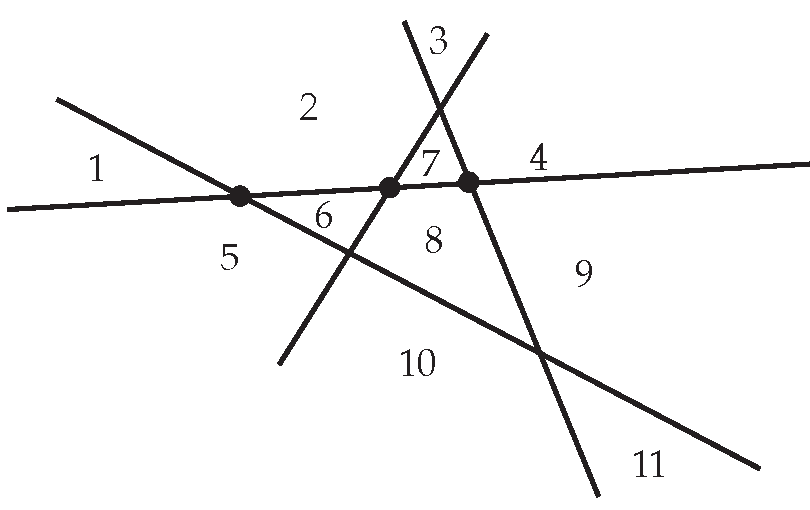
\includegraphics[width=0.5\textwidth]{induction-figs/lines-regions}
    \caption{Lines and regions in the plane}
    \label{fig:induction:lines-regions}
  \end{figure}
  With the recursive formula, we thus have $r(5)=5+11=16$,
  $r(6)=6+16=22$ and $r(7)=7+22=29$. Even by hand, it wouldn't be all
  that much trouble to calculate $r(100)$.  We could do it before
  lunch.

\end{example}

\begin{example}
  A $2\times n$ checkerboard will be tiled with rectangles of size
  $2\times1$ and $1\times2$.  Find a recursive formula for the number
  $t(n)$ of tilings.  Clearly, $t(1)=1$ and $t(2)=2$.  When $n>2$,
  consider the rectangle that covers the square in the upper right
  corner.  If it is vertical, then preceding it, we have a tiling of
  the first $n-1$ columns.  If it is horizontal, then so is the
  rectangle immediately underneath it, and proceeding them is a tiling
  of the first $n-2$ columns.  This shows that $t(n)=t(n-1)+t(n-2)$.
  In particular, $t(3)=1+2=3$, $t(4)=2+3=5$ and $t(5)= 3+5=8$.
\end{example}

Again, if compelled, we could get $t(100)$ by hand, and a computer
algebra system could get $t(1000)$.

\begin{example}
  Call a ternary string \textit{good} if it never contains a $2$
  followed immediately by a $0$; otherwise, call it \textit{bad}. Let
  $g(n)$ be the number of good strings of length $n$. Obviously
  $g(1)=3$, since all strings of length $1$ are good.  Also, $g(2)=8$
  since the only bad string of length~$2$ is $(2,0)$.  Now consider a
  value of $n$ larger than~$2$.

  Partition the set of good strings of length~$n$ into three parts,
  according to the last character. Good strings ending in $1$ can be
  preceded by any good string of length $n-1$, so there are $g(n-1)$
  such strings. The same applies for good strings ending in $2$. For
  good strings ending in $0$, however, we have to be more careful. We
  can precede the $0$ by a good string of length~$n-1$ provided that
  the string does not end in $2$. There are $g(n-1)$ good strings of
  length~$n-1$ and of these, exactly $g(n-2)$ end in a~$2$.  Therefore
  there are $g(n-1)-g(n-2)$ good strings of length~$n$ that end in
  a~$0$.  Hence the total number of good strings of length~$n$
  satisfies the recursive formula $g(n) = 3g(n-1) - g(n-2)$.  Thus
  $g(3) = 3\cdot8 -3= 21$ and $g(4)= 3\cdot21-8= 55$.
\end{example}

Once more, $g(100)$ is doable by hand, while even a modest computer can be
coaxed into giving us $g(5000)$.

\subsection{Finding Greatest Common Divisors}\label{s:induction:gcd}

There is more meat than you might think to the following elementary
theorem, which seems to simply state a fact that you've known since
second grade.

\begin{theorem}[Division Theorem]\label{thm:division}
Let $m$ and $n$ be positive integers.  Then there exist
unique integers $q$ and $r$ so that
\[
m = q\cdot n+r\quad\text{and}\quad 0 \le r < n.
\]
We call $q$ the \emph{quotient} and $r$ the \emph{remainder}.
\end{theorem}

\begin{proof} 
We settle the claim for existence.  The uniqueness part is
just high-school algebra.  If the theorem fails to hold, then
let $t$ be the least positive integer for which there are
integers $m$ and $n$ with $m+n=t$, but there
do not exist integers $q$ and $r$ with $m=qn+r$ and $0\le r<n$.

First, we note that $n\neq 1$, for if $n=1$, then we could take
$q=m$ and $r=0$.  Also, we cannot have $m=1$, for if $m=1$, then
we can take $q=0$ and $r=1$.  Now the statement holds for the
pair $m-1$, $n$ so there are integers $q$ and $r$ so that

\[
m-1 = q\cdot n+r\quad\text{and}\quad 0 \le r < n.
\]
Since $r<n$, we know that $r+1\le n$.  If $r+1<n$, then
\[
m = q\cdot n+(r+1)\quad\text{and}\quad 0 \le r+1 < n.
\]
On the other hand, if $r+1=n$, then
\[
m = q\cdot n+(r+1)=nq+n=(q+1)n=(q+1)n+0.
\]
The contradiction completes the proof.
\end{proof}

Recall that an integer $n$ is a \emph{divisor} of an integer $m$ if
there is an integer $q$ such that $m=qn$. (We write $n\mid m$ and read
``$n$ divides $m$''.) An integer $d$ is a \emph{common divisor} of
integers $m$ and $n$ if $d$ is a divisor of both $m$ and $n$. The
\emph{greatest common divisor} of $m$ and $n$, written $\gcd(m,n)$, is
the largest of all the common divisors of $m$ and $n$.

Here's a particularly elegant application of the preceding basic
theorem:

\begin{theorem}[Euclidean Algorithm]\label{thm:euclideanalg}
Let $m,n$ be positive integers and let $q$ and $r$ be
the unique integers for which
\[
m = q\cdot n+r\quad\text{and}\quad 0 \le r < n.
\]
If $r>0$, then $\gcd(m,n)=\gcd(n,r)$.
\end{theorem}
\begin{proof}
  Consider the expression $m=q\cdot n+r$, which is equivalent to
  $m-q\cdot n = r$. If a number $d$ is a divisor
  of $m$ and $n$, then $d$ must also divide $r$.  Similarly, if $d$ is
  a divisor of $n$ and $r$, then $d$ must also divide $m$.
\end{proof}

Here is a code snippet that computes the greatest common divisor of
$m$ and $n$ when $m$ and $n$ are positive integers with $m\ge n$.  We
use the familiar notation $m\%n$ to denote the remainder $r$ in the
expression $m=q\cdot n+r$, with $0\le r < n$.

\medskip
\begin{tt}
\noindent
int gcd(int m, int n) \{\\
\hspace{.25in}\mbox{} if (m\%n == 0) return n;\\
\hspace{.25in}\mbox{} else return gcd(n, m\%n);\\
\}\\
\end{tt}

\medskip The disadvantage of this approach is the somewhat wasteful
use of memory due to recursive function calls. It is not difficult to
develop code for computing the greatest common divisor of $m$ and $n$
using only a loop, i.e., there are no recursive calls. With minimal
extra work, such code can also be designed to solve the following
diophantine equation problem:

\begin{theorem}\label{thm:gcd-dioph}
  Let $m$, $n$, and $c$ be positive integers.  Then there exist
  integers $a$ and $b$, not necessarily non-negative, so that
  $am+bn=c$ if and only if $c$ is a multiple of the greatest common
  divisor of $m$ and $n$.
\end{theorem}

Let's see how the Euclidean algorithm can be used to write $\gcd(m,n)$
in the form $am+bn$ with $a,b\in\ints$ with the following example.

\begin{example}
  Find the greatest common divisor $d$ of $3920$ and $252$ and find
  integers $a$ and $b$ such that $d=3920a+252b$.

  In solving the problem, we demonstrate how to perform the Euclidean
  algorithm so that we can find $a$ and $b$ by working
  backward. First, we note that
  \[3920 = 15\cdot 252 + 140.\]
  Now the Euclidean algorithm tells us that
  $\gcd(3920,252)=\gcd(252,140)$, so we write
  \[252 = 1\cdot 140 + 112.\]
  Continuing, we have $140= 1\cdot 112 + 28$ and $112 = 4\cdot 28+0$,
  so $d=28$. 

  To find $a$ and $b$, we now work backward through the equations we
  found earlier, ``solving'' them for the remainder term and then
  substituting. We begin with
  \[28 = 140-1\cdot 112.\]
  But we know that $112=252-1\cdot 140$, so
  \[28=140-1(252-1\cdot 140) = 2\cdot 140 - 1\cdot 252.\]
  Finally, $140 = 3920-15\cdot 252$, so now we have
  \[28= 2(3920-15\cdot 252) - 1\cdot 252 = 2\cdot 3920-31\cdot 252.\]
  Therefore $a=2$ and $b=-31$.
\end{example}

\subsection{Sorting}

One of the most common and most basic computing problems is sorting:
Given a sequence $a_1,a_2,\dots,a_n$ of $n$ distinct integers,
rearrange them so that they are in increasing order.  We describe
here an easy recursive strategry for accomplishing this task.  This
strategy is known as \textit{Merge Sort}, and it is one of several
optimal algorithms for sorting.  Introductory computer science
courses treat this topic in greater depth.  In our course, we simply
need some good strategy and merge sort works fine for our purposes.

To present merge sort, must first develop a strategy for solving a 
special case of the sorting problem.
Suppose we have two $s+t$ distinct integers
$\{u_1,u_2,\dots,u_s,v_1,v_2,\dots,v_t\}$ with $u_1<u_2<\dots<u_s$
and $v_1<v_2<\dots<v_t$.  How do we \textit{merge} these two sequences
into a single increasing sequence of length $s+t$.
Imagine the two sequences placed on two horizontal lines, one immediately
under the other.  Then let $u$ be the least integer in the first
sequence and $v$ the least integer in the second.  At the moment,
this implies that $u=u_1$ and $v=v_1$, but integers will be deleted 
from the two sequences as the process is carried out.  Regardless, the 
meaning of $u$ and $v$ will be preserved.   Also, set $n=1$.
Then take $a_n$ as the minimum of $u$ and $v$ and delete $a_n$ from
the sequence in which it occurs.  Then increase $n$ by $1$ and
repeat.  Here is a code snippet for accomplishing a merge operation,
with $u_p$ now written as $u[p]$.  

\medskip
\begin{tt}
\noindent
p = q = 1;
for (i = 1; i < s+t+1; i++) \{\\
a[i] = min(u[p], v[q]);\\
if (min(u[p], v[q])==u[p]) p = p+1;\\
\quad  else q = q+1;\\
\}\\
\end{tt}

Now that we have a good strategy for merging, it is easy to
develop a recursive strategy for sorting.  Given a sequence
$a_1,a_2,\dots,a_n$ of $n$ distinct integers, we set $s=\lceil n/2\rceil$
and $t=\lfloor n/2\rfloor$.  Then let $u_i=a_i$ for $i=1,2,\dots,s$ and
$v_j=a_{s+j}$, for $j=1,2,\dots,t$.  Sort the two subsequences
and then merge them.  For a concrete example, given the
sequence $(2,8,5,9,3,7,4,1,6)$, we split into $(2,8,5,9,3)$ and
$(7,4,1,6)$.  These subsequences are sorted (by a recursive call)
into $(2,3,5,8,9)$ and $(1,4,6,7)$, and then these two sorted
sequences are merged.

For running time, if $S(n)$ is the number of operations it takes
to sort a sequence of $n$ distinct integers, then $S(2n)\le2 S(n) + 2n$,
since it clearly takes $2n$ steps to merge two sorted sequences
of length $n$.  This leads to the bound  $S(n) = O(n\log n)$,
and in computer science courses, you will learn (here it is an
exercise) that this is optimal.

\section{Mathematical Induction}\label{s:induction:induction}

Now we move on to induction, the powerful twin of recursion.

Let $n$ be a positive integer. Consider the following mathematical 
statements, each of which involve $n$:

\begin{enumerate}
\item $2n+7 = 13$.
\item $3n-5=9$.
\item $n^2-5n+9=3$.
\item $8n-3 < 48$.
\item $8n-3 > 0$.
\item $(n+3)(n+2) =n^2+5n+6$.
\item $n^2 -6n + 13 \ge 0$.
\end{enumerate}

Such statements are called \textit{open} statements.  Open statements
can be considered as \textit{equations}, i.e., statements that are
valid for certain values of $n$.  Statement~1 is valid only when
$n=3$.  Statement~2 is never valid, i.e., it has no solutions among
the positive integers. Statement~3 has exactly two solutions, and
Statement~4 has six solutions.  On the other hand, Statements~5, 6
and~7 are valid for all positive integers.

At this point, you are probably scratching your head, thinking that
this discussion is trivial.  But let's consider some statements that
are a bit more complex.

\begin{enumerate}
\item The sum of the first $n$ positive integers is $n(n+1)/2$.
\item The sum of the first $n$ odd positive integers is $n^2$.
\item $n^n \ge  n! + 4,000,000,000n2^n$\quad when $n\ge 14$.
\end{enumerate}

How can we establish the validity of such statements, provided of
course that they are actually true?  The starting point for providing
an answer is the following property:

\medskip 
\noindent\textbf{Principle of Mathematical Induction} Let $S_n$ be an open
statement involving a positive integer $n$.  If $S_1$ is true, and if
for each positive integer $k$, assuming that the statement $S_k$ is
true implies that the statement $S_{k+1}$ is true, then $S_n$ is true
for every positive integer~$n$.

\medskip With a little thought, you should see that the Principle of
Mathematical Induction is logically equivalent to the Well Ordered
Property of Positive Integers.  If you haven't already done so, now
might be a good time to look over \autoref{app:background} on background
material.
 
\section{Inductive Definitions}\label{s:induction:inductdefs}

Although it is primarily a matter of taste, recursive
definitions can also be recast in an inductive setting.
As a first example, set $1!=1$ and whenever $k!$ has
been defined, set $(k+1)!=(k+1)k!$.

As a second example, set
\[
\sum_{i=1}^1 f(i) = f(1)\quad\text{and}\quad
 \sum_{i=1}^{k+1} f(i)= \sum_{i=1}^{k} f(i)+ f(k+1) 
\]
In this second example, we are already using an abbreviated
form, as we have omitted some English phrases. 
But the meaning should be clear.

Now let's back up and give an example which would really
be part of the development of number systems.  Suppose
you knew everything there was to know about the \textit{addition}
of positive integers but had never heard anything about
\textit{multiplication}.  Here's how this operation can
be defined. 

Let $m$ be a positive integer.  Then set
\[
m\cdot1 = m\quad\text{and}\quad m\cdot(k+1)=m\cdot k+ m
\]
You should see that this \textit{defines} multiplication
but doesn't do anything in terms of establishing such
familiar properties as the commutative and associative
properties.  Check out some of the details in \autoref{app:background}. 

\section{Proofs by Induction}\label{s:induction:proofs}

No discussion of recursion and induction would be
complete without some obligatory examples of proofs using
induction.  We start with the ``Hello World'' example. 

\begin{proposition}\label{prop:sumints}
  For every positive integer $n$, the sum of the first $n$ positive
  integers is $n(n+1)/2$, i.e.,
\[
\sum_{i=1}^n i=\frac{n(n+1)}{2}.
\]
\end{proposition}

For our first version of a proof of
\hyperref[prop:sumints]{Proposition~\ref*{prop:sumints}}, we clearly
identify the open statement $S_n$ and describe the proof carefully in
terms of $S_n$. As you develop more experience with writing proofs by
induction, this will become less essential, as you'll see in the
second version of the proof.

\begin{proof}[First proof]
  Let $n$ be a positive integer, and let $S_n$ be the open statement 
  \[\sum_{i=1}^n i = \frac{n(n+1)}{2}.\]
  We will prove that $S_n$ is true for all positive integers by
  induction. For the basis step, we must prove that $S_1$ is
  true. When $n=1$, the left-hand side of $S_n$ is just $1$, while the
  right-hand side evaluates to $1(1+1)/2=1$. Therefore, $S_1$ is true.

  Next we assume that for some positive integer $k$, $S_k$ is
  true. That is, we assume 
  \[
  \sum_{i=1}^k i=\frac{k(k+1)}{2}.
  \]
  We now seek to prove that $S_{k+1}$ is true, and begin by
  considering the left-hand side of $S_{k+1}$. We notice that
  \[
  \sum_{i=1}^{k+1}i=\left(\sum_{i=1}^k i\right) +(k+1)=
  \frac{k(k+1)}{2}+(k+1),\]
  since our inductive hypothesis that $S_k$ is true gives us the
  simpler formula for the summation. Now continuing with a bit of
  algebra, we find
  \[\frac{k(k+1)}{2}+(k+1)=\frac{k^2+3k+2}{2}=\frac{(k+1)(k+2)}{2}.
  \]
  Therefore, $S_{k+1}$ is true.  Since we have shown that $S_1$ is
  true and that for every positive integer $k$, if $S_k$ is true,
  then $S_{k+1}$ is true, we conclude that $S_n$ is true for all
  positive integers $n$ by the Principle of
  Mathematical Induction.
\end{proof}

Before looking at a refined version of this proof, let's take a moment
to discuss the key steps in every proof by induction. The first step
is the \emph{basis step}, in which the open statement $S_1$ is shown to be
true. (It's worth noting that there's nothing special about $1$
here. If we want to prove only that $S_n$ is true for all integers
$n\geq 5$, then proving that $S_5$ is true is our basis step.) When
proving the basis step, if $S_n$ is an equation, we do not just write
down $S_1$ and move on. We need to \emph{prove} that $S_1$ is
true. Notice how in the proof above, we discussed the left-hand side
of $S_1$ and the right-hand side of $S_1$ and concluded that they were
equal.

After the basis step comes the \emph{inductive step}, in which we
assume that $S_k$ is true for \textbf{some} positive integer $k$ and
prove that $S_{k+1}$ is true. When doing this, we call $S_k$ our
\emph{inductive hypothesis}. In the inductive step, the most common
mistake students make is starting with the entirety of $S_{k+1}$ and
manipulating it until they obtain a true statement. This is dangerous,
as it is possible to start with something false and through valid
algebraic steps, obtain a true statement. Instead, the best option is
to work as with the basis step: if $S_{k+1}$ is an equation or inequality,
work on one side until you find a place to apply the inductive
hypothesis and then continue until you obtain the other side. If the
algebra gets tricky along the way, you can also work with the
left-hand side of $S_{k+1}$ and separately work with the right-hand side of
$S_{k+1}$. If you're able to manipulate both sides to be in the same
form, then you have shown they are equal and $S_{k+1}$ is true.

Now let's take a look at a more refined proof of
\hyperref[prop:sumints]{Proposition~\ref*{prop:sumints}}. From here
on, when we give a proof by induction, we'll use this style. As you're
getting started with induction proofs, you may find it useful to be
more explicit about the steps as we did in the first proof above.

\begin{proof}[Refined proof]
  We first prove the assertion when $n=1$.  For this value of $n$, the
  left-hand side is just~$1$, while the right-hand side evaluates to
  $1(1+1)/2=1$.

  Now assume that for some positive integer $k$, the formula holds
  when $n=k$, i.e., assume that
  \[
  \sum_{i=1}^k i=\frac{k(k+1)}{2}.
  \]
  Then it follows that
  \[
  \sum_{i=1}^{k+1}i=\left(\sum_{i=1}^k i\right) +(k+1)=
  \frac{k(k+1)}{2}+(k+1)=\frac{k^2+3k+2}{2}=\frac{(k+1)(k+2)}{2}.
  \]
  Thus the formula also holds when $n=k+1$.  By the Principle of
  Mathematical Induction, it holds for all positive integers $n$.
\end{proof}

The preceding arguments are 100\% correct\dots but some combinatorial
mathematicians would argue that they may actually hide what is really
going on.  These folks would much prefer a combinatorial proof, as was
provided in the preceding chapter.  Our perspective is that you should
prefer to give a combinatorial proof---when you can find one.  But if
pressed, you should be able to give a formal proof by mathematical
induction.

Here's a second example, also quite a classic.  Again, recall that we
gave a combinatorial proof in the last chapter. As you read the proof,
make sure you can identify the open statement $S_n$, the basis step,
and the inductive step.

\begin{proposition}\label{prop:sumodd}
For each positive integer $n$, the
sum of the first $n$ odd positive integers is $n^2$, i.e.,
\[
\sum_{i=1}^n (2i-1)= n^2.
\]
\end{proposition}
\begin{proof}
We will prove this by induction. First, note that the formula holds when
$n=1$.  Now suppose that $k$ is a positive integer and
that the formula holds when $n=k$, i.e., assume
\[
\sum_{i=1}^k (2i-1)= k^2.
\]
Then
\[
\sum_{i=1}^{k+1}(2i-1)=\left(\sum_{i=1}^k 2i-1\right)+2k+1=
k^2+(2k+1)=(k+1)^2.
\]
Therefore, the proposition follows by the Principle of Mathematical Induction.
\end{proof}

Here's a more general version of the first result in
this section, and again we note that we gave a combinatorial
proof in the last chapter.

\begin{proposition}\label{prop:sum-bincoeffs}
Let $n$ and $k$ be non-negative integers with $n\ge k$.
Then
\[
\sum_{i=k}^n \binom{i}{k}=\binom{n+1}{k+1}.
\]
\end{proposition}
\begin{proof}
Fix a non-negative integer $k$.  We then prove the
formula by induction on $n$.  If $n=k$, note that
the left hand side is just $\binom{k}{k}=1$, while the
right hand side is $\binom{k+1}{k+1}$ which is also~$1$.
Now assume that $m$ is a non-negative integer, with 
$m\ge k$, and that the
formula holds when $n=m$, i.e., assume that
\[
\sum_{i=k}^m \binom{i}{k}=\binom{m+1}{k+1}.
\]

Then
\begin{align*}
\sum_{i=k}^{m+1}\binom{i}{k} &= \sum_{i=k}^{m}\binom{i}{k} +\binom{m+1}{k}\\
        &=\binom{m+1}{k+1}+\binom{m+1}{k}\\
        &=\binom{m+2}{k+1}.
\end{align*} 
Therefore, the proposition follows by the Principle of Mathematical Induction.
\end{proof}


\section{Strong Induction}\label{s:induction:strong-induction}

There are occasions where the Principle of Induction, at least
as we have studied it up to this point, does not seem sufficient.
Here is a concrete example.
The professor asked Bob to study a function  $f(n)$ defined recursively by
$f(n) = 2f(n-1) - f(n-2)$ with $f(1)=3$ and $f(2)=5$.  Specifically,
the professor asked Bob to compute $f(10^{10})$, which seems like 
a daunting task.  Over coffee, Bob scribbled on a napkin and determined
that $f(3)=7$ and $f(4)=9$, and on the basis of these calculations alone,
he thought that it might just be possible that  
$f(n) = 2n+1$ for all $n\geq 1$.  If this were true, he could
simply report that $f(10^{10})=2\cdot 10^{10}+1=20000000001$.

Bob was beginning to understand proofs by induction, so he tried to
prove that $f(n)=2n+1$ for all $n\ge1$ by induction. For the base step,
he noted that $f(1)= 3=2\cdot1+1$, so all is ok to this point.
For the inductive step, he assumed that $f(k)=2k+1$ for some $k\ge1$
and then tried to prove that $f(k+1)=2(k+1)+1$.  If this step could be completed,
then the proof by induction would be done.

But at this point, Bob seemed to hit a barrier, because 
\[f(k+1) = 2f(k) - f(k-1) = 2(2k+1) - f(k-1),
\]
using the inductive hypothesis to replace $f(k)$ by $2k+1$. However,
he's was totally perplexed about what to do with the $f(k-1)$.  If he knew
that $f(k-1)=2(k-1)+1$, then the right hand side
would result in $2(2k+1) -(2k-1)= 2k+3=2(k+1)+1$, which is
exactly what he wants.  Bob always plays by the rules, and he
has to admit that he doesn't know that $f(k-1)=2(k-1)+1$.  He
only knows that $f(k)=2k+1$.

Bob was about to throw in the towel and ask his computer to start
making the calculations recursively, when
Carlos comes along and asks what he's doing. Carlos sees right away
that the approach Bob was taking to prove that $f(n)=2n+1$ by induction
won't work---but after a moment's reflection, Carlos says that there's
a stronger form of an inductive proof that will do the trick.
Carlos patiently explained to Bob a proposition which is called the
\textit{Strong} Principle of Mathematical Induction.  To prove that
an open statement $S_n$ is valid for all $n\ge1$, it is enough to
(a)~Show that $S_1$ is valid, and (b)~Show that $S_{k+1}$ is valid
whenever $S_m$ is valid for all integers $m$ with $1\le m\le k$.

The validity of this proposition is trivial since it is \textit{stronger}
than the principle of induction.  What is novel here is that in order
to prove a statement, it is sometimes to your advantage to prove
something even stronger.  Combinatorial mathematicians call this
the ``bootstrap'' phenomenon.

Equipped with this observation, Bob saw clearly that the strong principle
of induction was enough to prove that $f(n)=2n+1$ for all $n\ge1$.
So he could power down his computer and enjoy his coffee.

\section{Discussion}\label{s:induction:discussion}
 
The group was debating the value of combinatorial proofs versus
formal proofs by induction.  Xing said that he actually preferred to
do a proof by induction, as a combinatorial proof, it could be
argued, wasn't really a proof.  Dave mumbled ``Combinatorial proofs
can always be made rigorous.''   They went back and forth for a
while and then Alice said ``But the professor never explained
that weird sequence

\[
1,2,3,4,1,2,3,4,5,1,2,3,4,5,2,3,4,5,6,2,3,4,5,6,1,2,3,4,5,2,3,4,5,6,\dots
\]
Dave was on a roll ``Who has change for a dollar?'' but nobody
understood why he would derail an argument over proofs when
everybody had already paid for the coffee.  Alice was more to the
point ``You know Dave, sometimes I just don't understand why
you say  the things you do.''  Dave smiled (maybe it was more of
a smirk) ``It's about making change.  The terms in this sequence
are the fewest number of coins required to make change.''
Bob said ``I don't get it.'' Dave continued ``The term  $a_n$ is
the fewest number of U.S. coins required to total to $n$ cents.''
Now everyone groaned, everyone except Carlos, who thought that
at least this time, Dave was really clever.

``Well'', said Bob ``that takes care of the strange sequence,
but I still don't see any difference between
induction and recursion.  Dave couldn't keep quiet ``No one does.''  Xing thought
differently and said ``In many programming languages, you try to
avoid recursion, preferring to use loops instead.  Otherwise, you
wind up overloading the stack.  As just one example, you can
compute the greatest common divisor $d$ of $m$ and $n$, as well as
find $a$ and $b$ so that $d=am+bn$ using a loop---with very
little storage.  The recursive approach discussed previously, with 
the inherent back tracking at the end, isn't really necessary.''  
Yolanda was impressed with Xing's extensive programming experience and 
knowledge, but Alice was less so.  

Zori was losing her patience and was especially grumpy today ``I don't
see any value to any of this stuff.  Who's going to pay me to find
greatest common divisors?''  Dave said ``Nobody.''  Alice said ``But
maybe there are some principles here that have practical application.''
Carlos joined in ``I think the basic principles behind establishing
that a computer program does what you intend have a lot to do with
induction and recursion.''  Bob said ``I don't understand.  When
I write a program, I just pay attention to details and after just 
a few corrections, they always work.''  Alice was brutal ``Maybe that's
because you don't do anything complicated.''  Carlos was more gentle
``Big software projects might have hundreds of thousands of lines
of code, and pieces of the final product might be written by
different groups of programmers at different moments in time.
Establishing correctness can be a very difficult task.''
Zori's ears perked up as she thought she saw something in
this last bit of conversation that might be a way to earn a salary.

\section{Exercises}\label{s:induction:exercises}

For questions asking you find a recursive formula, be sure to give
enough initial values to get the recursion going.


\begin{enumerate}\item  A database uses record identifiers that are alphanumeric
    strings in which the $10$ decimal digits and $26$ upper-case
    letters are valid symbols. The criteria that define a valid record
    identifier are recursive. A valid record identifier of length
    $n\geq 2$ can be constructed in the following ways:
    \begin{itemize}
    \item beginning with any upper-case letter other than $D$ and
      followed by any valid record identifier of length $n-1$;
    \item beginning with $1C$, $2K$, or $7J$ and followed by any valid
      record identifier of length $n-2$; or
    \item beginning with $D$ and followed by any string of $n-1$
      decimal digits.
    \end{itemize}
    Let $r(n)$ denote the number of valid record identifiers of length
    $n$. We take $r(0)=1$ and note that $r(1) = 26$. Find a recursion
    for $r(n)$ when $n\geq 2$ and use it to compute $r(5)$.
\item    Consider a $1\times n$ checkerboard. The squares of the
    checkerboard are to be painted white and gold, but no two
    consecutive squares may both be painted white. Let $p(n)$ denote
    the number of ways to to paint the checkerboard subject to this
    rule. Find a recursive formula for $p(n)$ valid for $n\geq 3$.
\item   Give a recursion for the number $g(n)$ of ternary strings of
    length $n$ that do not contain $102$ as a substring.

\item A $2\times n$ checkerboard is to be tiled using two types of
  tiles. The first tile is a $1\times 1$ square tile. The second tile
  is called an $L$-tile and is formed by removing the upper-right
  $1\times 1$ square from a $2\times 2$ tile. The $L$-tiles can be
  used in any of the four ways they can be rotated. (That is, the
  ``missing square'' can be in any of four positions.) Let $t(n)$
  denote the number of tilings of the $2\times n$ checkerboard using
  $1\times 1$ tiles and $L$-tiles. Find a recursive formula for $t(n)$ and
  use it to determine $t(7)$.
\item Let $S$ be the set of strings on the alphabet $\{0,1,2,3\}$ that
  do not contain $12$ or $20$ as a substring. Give a recursion for the
  number $h(n)$ of strings in $S$ of length $n$. \textit{Hint}: Check
  your recursion by manually computing $h(1)$, $h(2)$, $h(3)$, and
  $h(4)$.
  %Solution: $h(n)=4h(n-1)-2h(n-2)+h(n-3)$ with $h(1)=4$,
  %  $h(2)=14$, and $h(3)=49$ and h(4) = 172

\item Find $d=\gcd(5544,910)$ as well as integers $a$ and $b$ such
  that $5544a + 910 b = d$.
\item Find $\gcd(827,249)$ as well as integers $a$ and $b$ such that
  $827a+249b = 6$.
\item Let $a$, $b$, $m$, and $n$ be integers and suppose that
  $am+bn=36$. What can you say about $\gcd(m,n)$?
\item  (A challenging problem)  For
  each formula, give both a proof using the Principle of
  Mathematical Induction and a combinatorial proof. One of the two
  will be easier while the other will be more challenging.
  \begin{enumerate}
  \item $\displaystyle 1^2+2^2+3^2+\dots+ n^2= \frac{n(n+1)(2n+1)}{6}$
%  \item $\displaystyle\binom{n}{0}\binom{n}{n}+\binom{n}{1}\binom{n}{n-1}+
%    \binom{n}{2}\binom{n}{n-2}+\dots+\binom{n}{n}\binom{n}{0}=\binom{2n}{n}$
  \item $\displaystyle\binom{n}{0}2^0+\binom{n}{1}2^1+\binom{n}{2}2^2+\dots+\binom{n}{n}2^n=3^n$
  \end{enumerate}
\item Show that for all integers $n\geq 4$, $2^n < n!$.
\item Show that for all positive integers $n$,
  \[\sum_{i=0}^n 2^i = 2^{n+1}-1.\]
\item Show that for all positive integers $n$, $7^n-4^n$ is divisible
  by $3$.
\item Show that for all positive integers $n$, $9^n-5^n$ is divisible
  by $4$.
\item It turns out that if $a$ and $b$ are positive integers with
  $a>b+1$, then there is a positive integer $M>1$ such that $a^n-b^n$
  is divisible by $M$ for all positive integers $n$. Determine $M$ in
  terms of $a$ and $b$ and prove that it is a divisor of $a^n-b^n$ for
  all positive integers $n$.
\item Use mathematical induction to prove that for all integers $n\geq
  1$,
  \[n^3 + (n+1)^3 + (n+2)^3\]
  is divisible by $9$.
\item Give a proof by induction of the Binomial Theorem
  (\autoref{thm:binomial}). How do you think it compares to the
  combinatorial argument given in \autoref{ch:strings}?
\item Consider the recursion given by $f(n) = 2f(n-1) - f(n-2) + 6$
  for $n\geq 2$ with $f(0)=2$ and $f(1)=4$. Use mathematical induction
  to prove that $f(n) = 3n^2-n+2$ for all integers $n\geq 0$.
\item Consider the recursion given by $f(n) = f(n-1)+f(n-2)$ for
  $n\geq 3$ with $f(1)=f(2)=1$. Show that $f(n)$ is divisible by $3$
  if and only if $n$ is divisible by $4$.
\item Suppose that $x\in\reals$ and $x>-1$. Prove that for all
  integers $n\geq 0$, $(1+x)^n\geq 1+nx$.
\item Show that there is a positive constant $c$ so that any algorithm 
 that sorts a sequence of $n$ positive integers must, in worst case, take 
 $cn\log n$ steps. \emph{Hint}:  There are $n!$ permutations of a set of $n$
 distinct integers.  Each operation reduces the number of possibilities
 by a multiplicative fraction which is at most $1/2$.  So if there
 are $t$ operations, then $2^t\ge n!$.  Now look up Stirling's
 approximation for $n!$ and continue from there.
\end{enumerate}

%%% Local Variables: 
%%% mode: latex
%%% TeX-master: "chap-skel-mtk"
%%% End: 
